%!TEX root = cscw2019-comic.tex
\section{Study on Persuasion: Results}
\label{sec:Study on Behavior Results}

In this section, we will first present the raw data used in the analysis, then introduce the Bayesian Model we used for data analysis and our analysis result.

\subsection{Raw Data}
\label{sub:Study on Behavior Raw Data}
In total we have 307 participants joined our study, 101 participants received the message in the text form, 102 participants received the same message in the comic form, and 104 participants received the comic message with social-proof. We ran an outlier analysis on participants' completion time and removed 30 participants from our dataset. The following analysis is based on a dataset with 277 participants, 91 of them is in pure-text condition, 97 of them is in comic condition, and 92 of them is in comic-social-proof condition. Of those 277 participants, 150 were self-identified as male, and 126 were self-identified as female, 1 participant chose not to disclose. 197 participants earned at least college degree.~\Cref{fig:contributions across conditions} compares the distributions of the charitable donations across the three conditions.

\begin{figure*}[htb]
	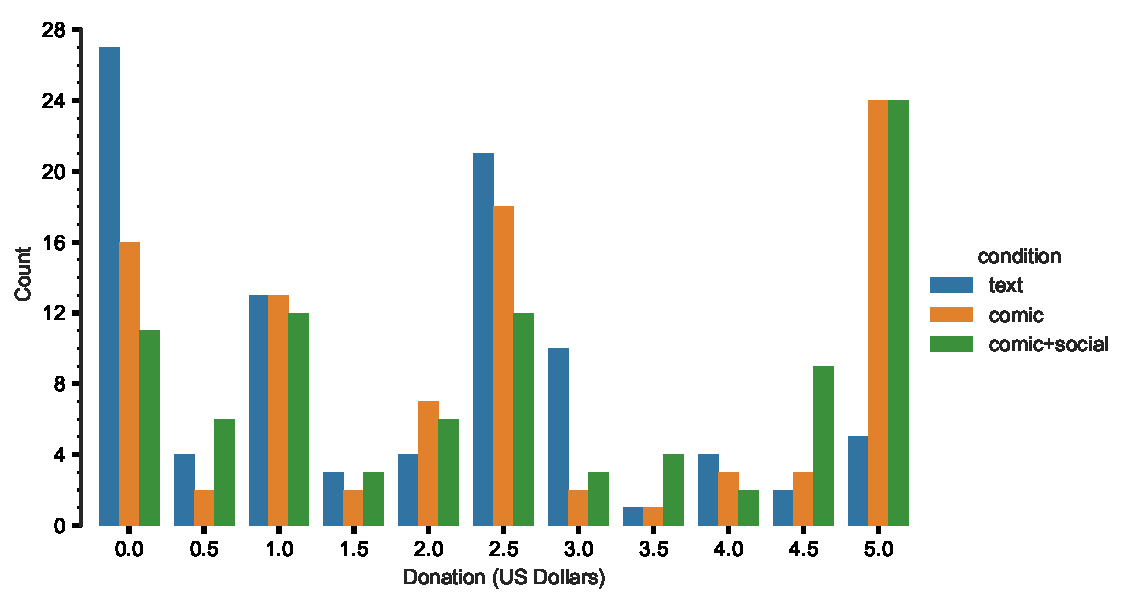
\includegraphics[width=1\textwidth]{./hari-code/contributions_across_conditions.pdf}
    \caption{The distribution of the amount of money participants decide to donate to the charity in each of the three conditions: text only; comic; comic with social norm.}
	\label{fig:contributions across conditions}
\end{figure*}



% \begin{figure*}[htb]
% 	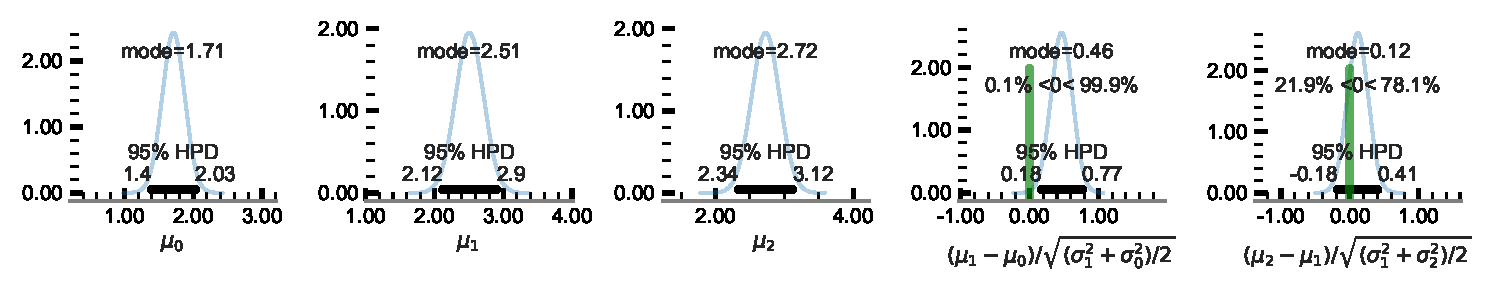
\includegraphics[width=1\textwidth]{./hari-code/new_exp_text_v_comic_v_social.pdf}
%     \caption{The posterior distribution of the amount of money participants decide to donate to the charity in each of the three conditions: text only ($\mu_0$); comic ($\mu_1$); comic with social norm ($\mu_2$). The right two panels are respectively: posterior distribution of the effect size contrasting the comic condition ($\mu_1$) and text ($\mu_0$); the effect size contrasting comic with social norm ($\mu_2$) with the plain comic ($\mu_1$). First notice that $\mu_2 > \mu_1 > \mu_0$. Furthermore, the modal effect size of comparing the comic panel against text is 0.48, a medium effect and the HPD interval $[0.17, 0.77]$ reliably excludes a ROPE of $[0 \pm 0.1]$, indicating that the effect is meaningful. The effect of introducing the social norm into the comic has a minor effect (mode=0.12) when contrasted against the plan comic, and the HPD interval $[-0.17, 0.41]$ includes a ROPE of $[0 \pm 0.1]$, indicating that the outcome is not convincing.}
% 	\label{fig:main-experiment2-effect}
% \end{figure*}


\subsection{Bayesian Formulation}
\label{sub:Bayesian Formulation}
We use a Bayesian formulation of the problem of identifying suitable predictors for the messages in comic form.~\textcite{Kay2016} provide an nice introduction on the appropriateness of Bayesian analysis for the HCI community. Bayesian analysis is attractive in our experiment due to two advantages: shifting the conversation from ``did it work'' to ``how strong is the effect''; and benefits to small $n$ studies.

Bayesian inference can sometimes differ from say a standard $t$-test widely used to compare two groups in the standard Null Hypothesis Significance Testing (NHST) framework. This is because the $t$-test assumes that the two populations from which samples are drawn, follow a Normal distribution, an assumption that can be violated in practice. Non-Normality is easily accounted for in a Bayesian formulation and~\textcite[][p. 470]{Kruschke2014} points out that the Normality assumption is one explanation why a $t$-test may be less sensitive to differences than a Bayesian analysis.

Our experiment has three experimental groups: text, comic and comic with social norm. One way to use classical statistical analysis for multiple groups would be to use ANOVA to see if the treatment (the use of comic) has any effect. However, ANOVA assumes equal variances within groups, and that the response within each group is Normally distributed.  It is straightforward in Bayesian Analysis to relax both assumptions: equal variances and Normality.

\begin{figure*}[htb]
	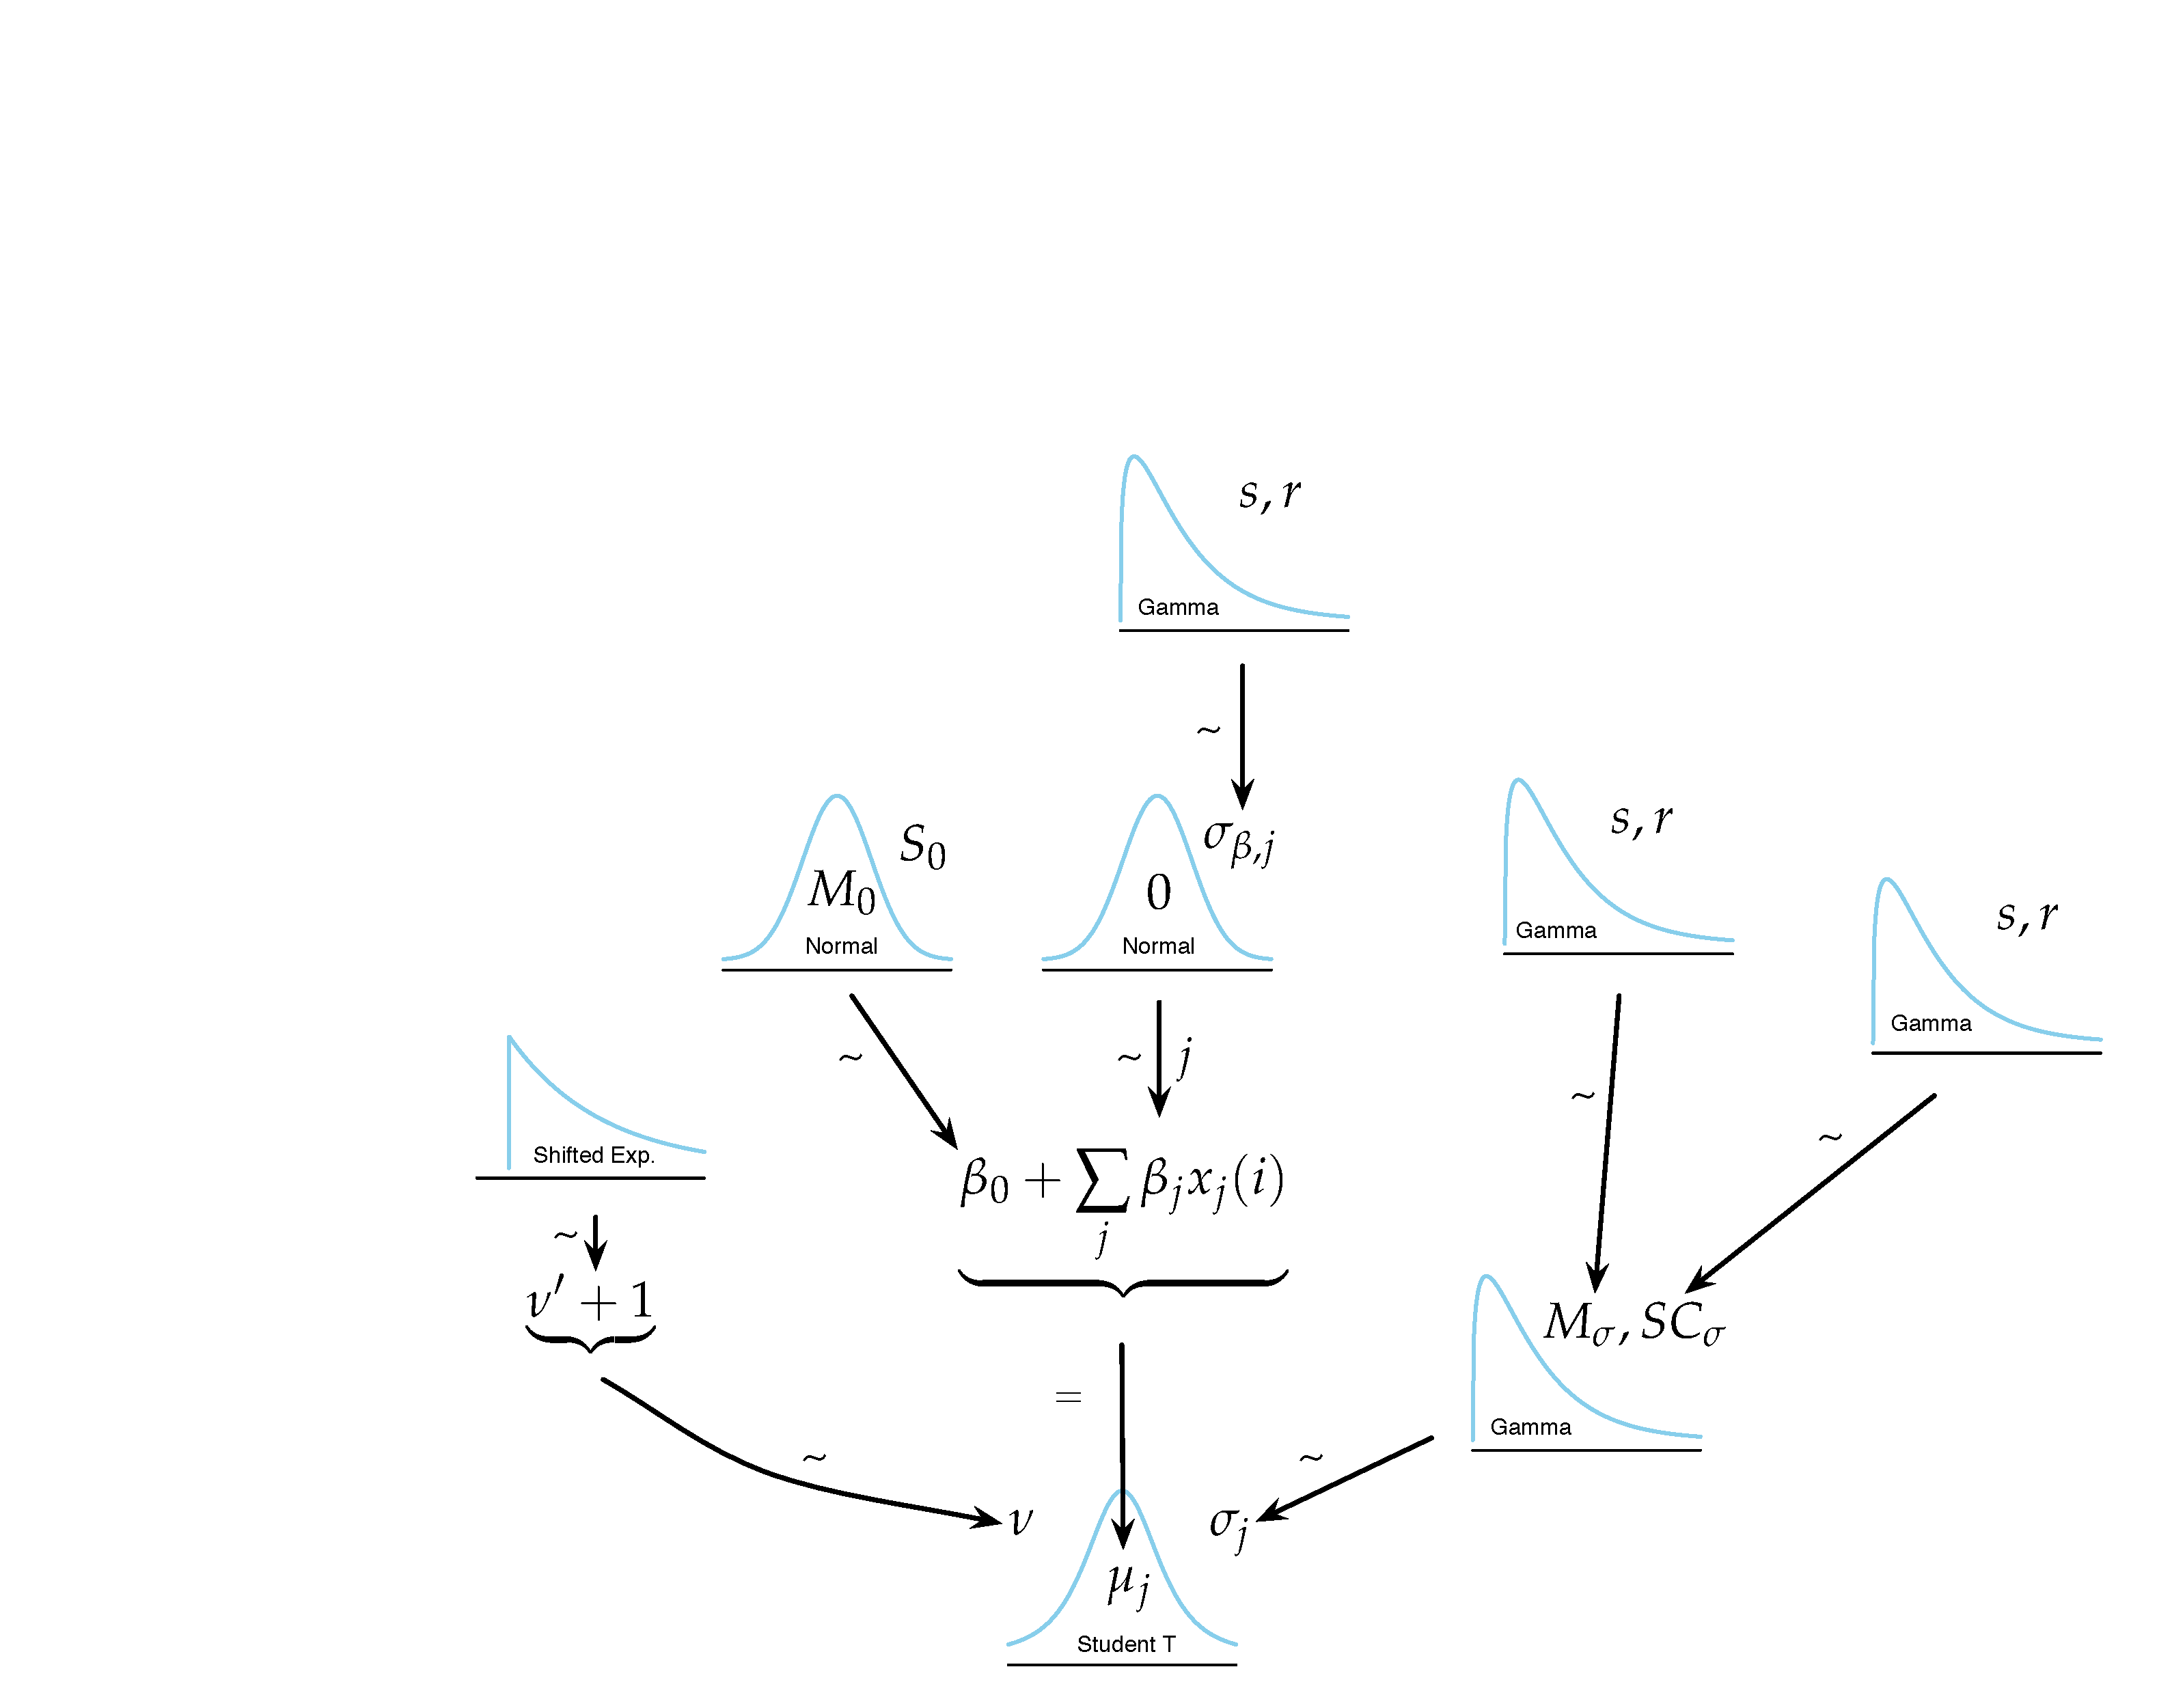
\includegraphics[width=1\textwidth]{./figures/gen_model.pdf}
    \caption{Our proposed Hierarchical Bayesian model.}
	\label{fig:generative model}
\end{figure*}



Now, we discuss our Bayesian formulation (see~\Cref{fig:generative model} for a graphical view of the model). There is one outcome variable $y_{i \mid j}$, the amount of donation to the charity by each participant $i$, under experimental condition $j$: text, comic, and comic with social norm. Our Bayesian model:

\begin{align}
    y_{i \mid j} \sim &  \mathrm{StudentT}(\nu, \mu_j, \sigma_j), \label{eq:bayesian formulation}\\
    \nu \sim & 1 + \exp(\lambda), \\
    \mu_j \sim & \beta_0 + \sum_j \beta_j x_j(i), \label{eq:mean response}\\
    \sigma_j \sim & \Gamma(M_{\sigma, j}, SC_{\sigma, j}),\\
    M_{\sigma, j} \sim & \Gamma(s,r), \\
    SC_{\sigma, j} \sim & \Gamma(s,r), \\
    \beta_0 \sim & N(M_0, SD_0), \\
    \beta_j \sim & N (0, \sigma_{\beta, j}), \\
    \sigma_{\beta, j} \sim & \Gamma(s,r).
\end{align}

\Cref{eq:bayesian formulation} says that the response $y_{i \mid j}$ of each group $j$ is modeled as a $\mathrm{StudentT}$ distribution with mode $\mu_j$,  scale $\sigma_j$ and with $\nu$ degrees of freedom; notice that this is a \textit{drawing distribution}, not the $t$-test. The $\mathrm{StudentT}$ allows us to model a non-Normal outcome with a heavy tail; assuming $y_{i \mid j}$ to be Normally distributed is equivalent to setting $\nu=\infty$. The degrees of freedom $\nu$ is drawn from a shifted exponential distribution, to ensure $\nu \geq 1$; the mode $\mu_j$ corresponding to each group is drawn from a Normal distribution with $\mu_j = \beta_0 + \sum_j \beta_j x_j(i)$, where the group indicator variable $x_j(i)=1 \iff \text{subject } i \text{ belongs to group } j$. The scale $\sigma_j$ of the normal distribution is drawn from a Gamma distribution $\Gamma(M_{\sigma, j}, SC_{\sigma, j})$, with mode $M_{\sigma, j}$ and scale $SC_{\sigma, j}$. The mode $M_{\sigma, j}$ and scale $SC_{\sigma, j}$ are each drawn from two independent Gamma distributions $\Gamma(s,r)$ with shape parameter $s$ and rate parameter $r$. The overall group response $\beta_0$ is modeled as a Normal distribution with mean $\mu_0$ and variance $\sigma_0$. For each of the $\beta_j$ for each group $j$ in~\Cref{eq:mean response}, $\beta_j$ is Normally distributed with mean $\mu=0$ and $\sigma_{\beta, j}$ drawn from a Gamma distribution $\Gamma(s,r)$ with shape parameter $s$ and rate parameter $r$. The random variables $\beta_j$ are centered around $\mu=0$ so that the group responses are modeled as deflections around the overall mean $\beta_0$. 

~\Cref{fig:generative model} indicates that we draw all the variances $\sigma_{\beta, j}$ from a Gamma $\Gamma(s,r)$ distribution, where $s$ refers to the shape parameter and $r$ refers to the rate parameter. We set the variables $s,r$ to allows a wide range of values for $\sigma_{\beta, j}$. Notice that we draw the variances $\sigma_{\beta, j}$ of each group $j$ independently from a \textit{common} Gamma distribution, implying that the variances (equivalently, the extent of deflections from the mean) for each predictor $\beta_j$ can be different. The main advantage of using a Gamma distribution is that we can specify a non-zero mode, important in controlling shrinkage in hierarchical models. By drawing the standard deviation variables $\sigma_{\beta, j}$ from a common Gamma distribution, the values of each element of $\beta_j$ informs the other elements. The ``information sharing'' among variables common to hierarchical Bayesian models and is an important reason why Bayesian models work so well with small datasets\footnote{The sharing of information causes the variance of each individual parameter $\beta_{j}$ to move towards the group variance, a phenomena known as ``shrinkage.'' }.

% The result ~\Cref{fig:main-experiment2-effect} shows the modal effect size between abstract-comic v. pure-text = 0.48; There is no overlap of the 95\% high probability density (HPD) interval with the ROPE of [-0.1, 0.1]. Thus the effect is of medium size and meaningful; the effect size between abstract-comic and social-proof-comic is 0.12; but since the distribution includes a ROPE of $[-0.1 \pm 0.1]$, the effect is not convincing.

\subsection{Analysis}
\label{sub:Analysis}

We analyzed the data using PyMC3~\cite{Salvatier2016}, a popular framework for Bayesian inference. Computational techniques for Bayesian inference use a stochastic sampling technique called Markov Chain Monte Carlo (MCMC) that samples the posterior distribution $P(\theta | D)$, where we want to estimate the parameters $\theta$ given the observations $D$. In particular, we used the Metropolis-Hastings sampler. The Gelman-Rubin statistic $\hat{R}$ was around 1, indicating that the different sampling chains converged. Furthermore, the effective sample size of all parameters was greater than 10,000.

\begin{figure*}[htb]
	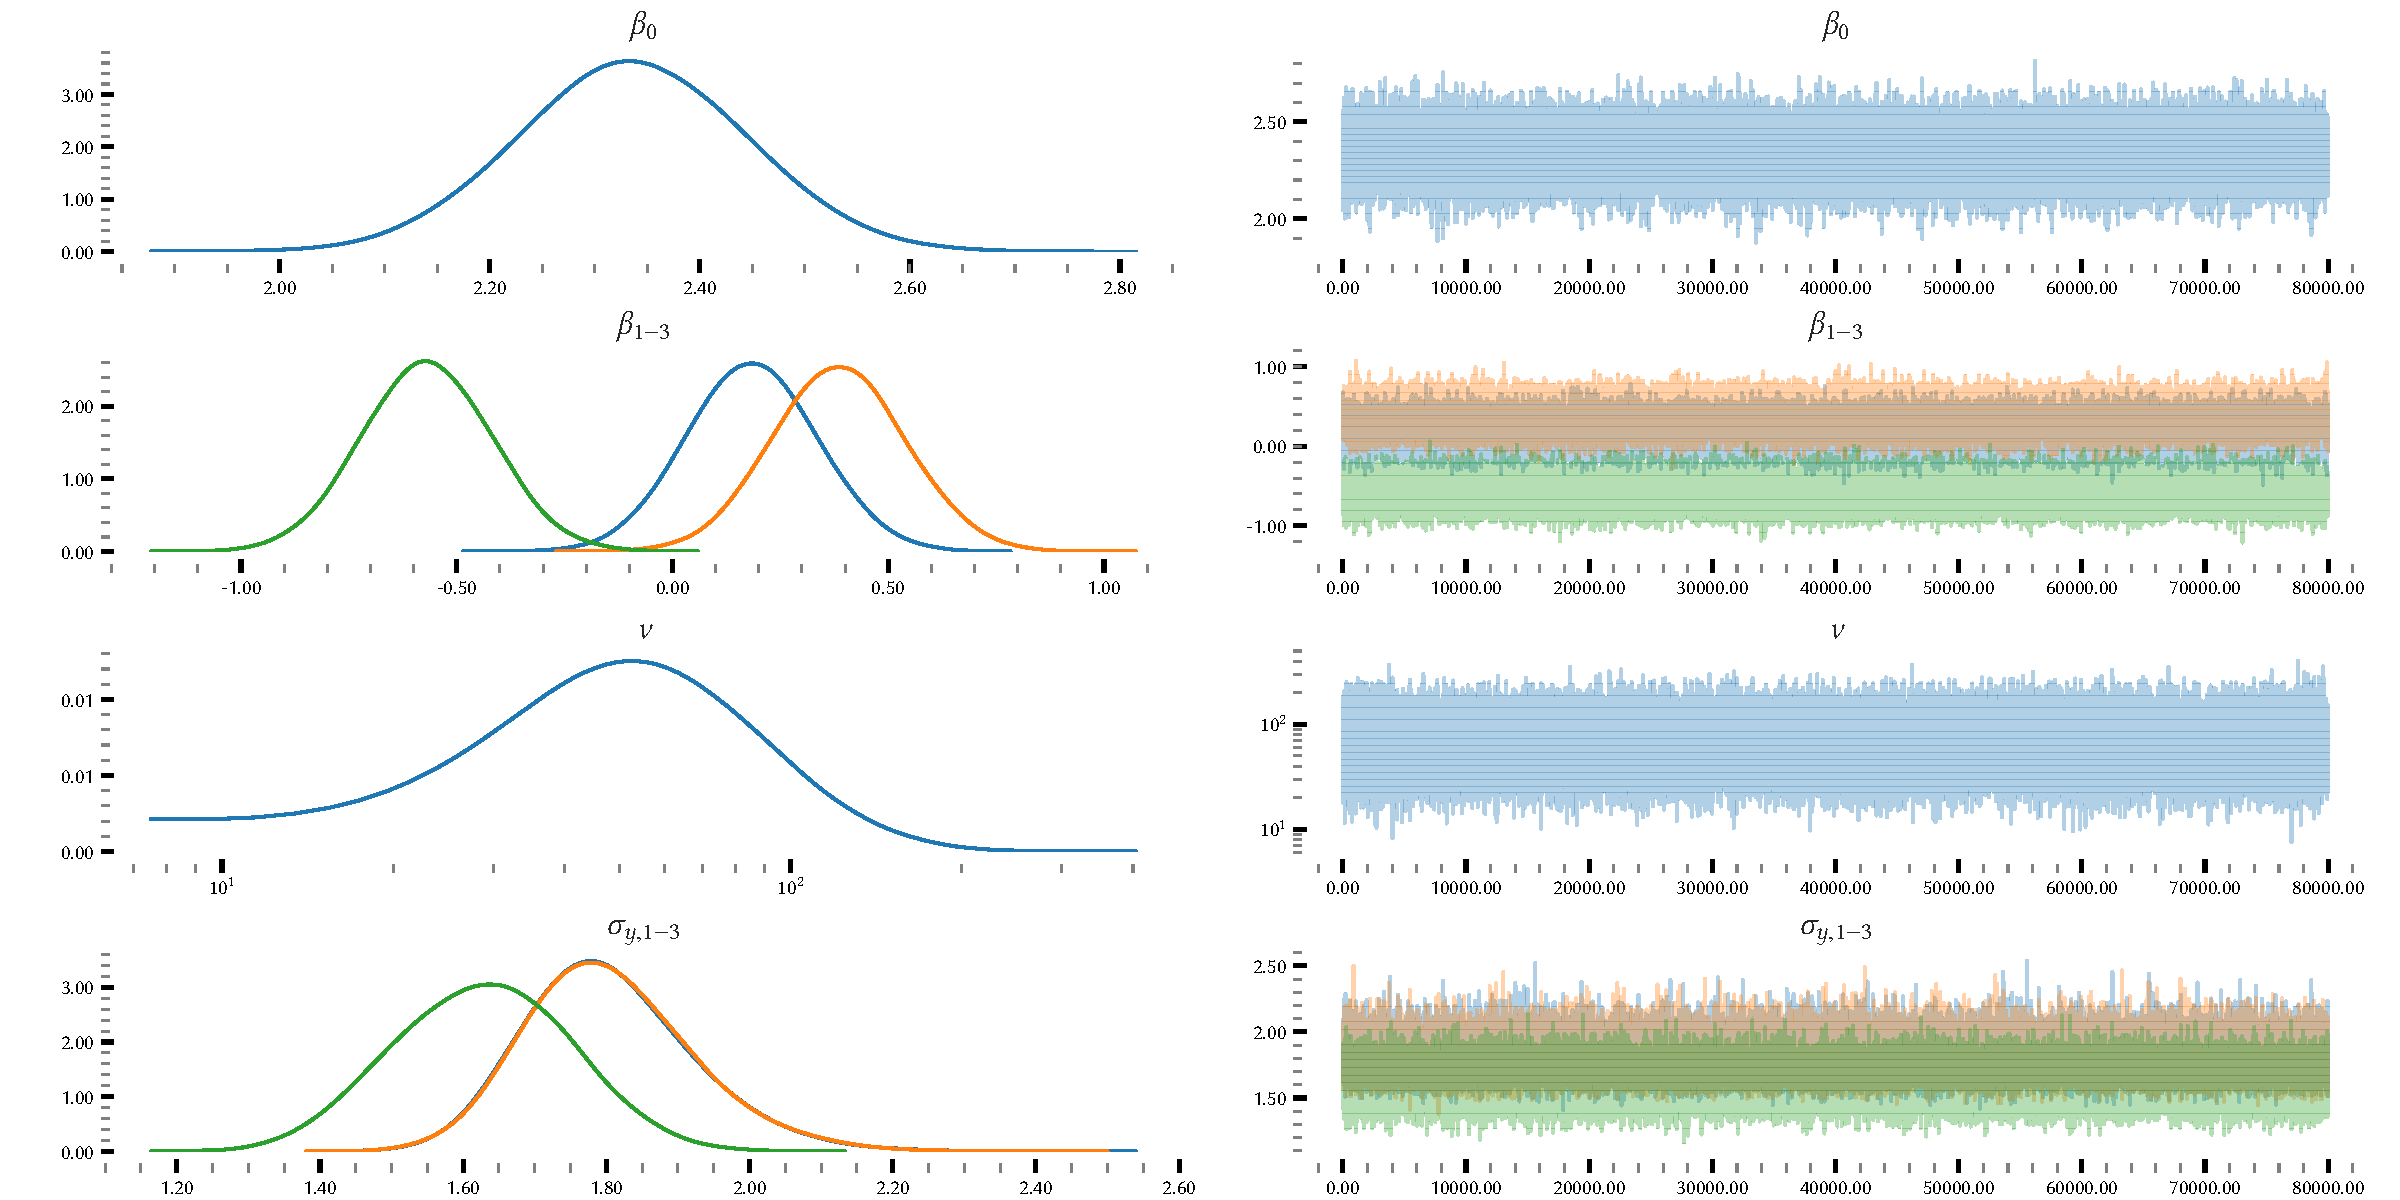
\includegraphics[width=1\textwidth]{./hari-code/robust_traceplot.pdf}
    \caption{Traceplot showing the results of the MCMC estimation. Left column shows the posterior distributions for $\beta_0, \beta_{[1-3]}, \nu, \sigma_{[1-3]}$, while the right column shows the corresponding traces. The posterior plots for $\nu$, the parameter corresponding to degrees of freedom has a modal value of $\nu=53$. While the ideal case of $\nu=\infty$ makes the StudentT distribution equivalent to the Normal distribution, in practice $\nu \geq 30$ is used to test for Normality. Thus the response distributions $y_{i \mid j}$ tend towards Normality. Notice that the mean of $\sigma_2$ (green curve, fourth panel, left column), variance of the group response in the case of text, is less than $\sigma_1$ or $\sigma_3$ (variances of the group responses for the comic, comic+social norm cases respectively), justifying our modeling assumptions of unequal variances across groups; the variances for the two comic conditions are nearly identical. The traces corroborate MCMC chain convergence. }
	\label{fig:traceplot}
\end{figure*}


In this section, we presented a Bayesian model to analyze the overall effect of using a abstract-comic to persuade people making charitable donation decisions, and understand the effect of adapting persuasive techniques in the abstract comic form. The results show that the use of abstract-comic produces a significant effect in persuading participants to donate. Although abstract-comic with social proof can produce larger effect, the contrast between abstract-comic and abstract-comic with social proof is not significant. Next we discuss the findings, limitations and design implications.
